\subsection{EU Nuclear Operation until 2050}

\begin{frame}
	\frametitle{Historical Operation of EU Reactors}

\begin{table}[h]
	\centering
	\scalebox{0.86}{
		\begin{tabular}{cccc}
			\hline
			\textbf{Category } & \textbf{Value} & \textbf{Unit} & \textbf{Specifics}\\ \hline
			Total UOX Usage  & 79,500 & MTHM &  \\ 
			Total MOX Usage  & 4,053 & MTHM & \\ 
			Total Used UOX Stored  & 110,013 & MTHM & \gls{UNF} that is not reprocessed\\  
			Total Used UOX Stored (France) & 22,824 & MTHM & \gls{UNF} that is not reprocessed \\
			Total Tails  & 1,086,903 & MTHM & \\ 
			Total Natural U Used  & 1,266,403 & MTHM & \\ \hline
		\end{tabular}}
		\caption{Simulation Results for Historical Nuclear Operation 
		of \gls{EU} Nations}
		\label{tab:sim_result}
\end {table}

\end{frame}

\begin{frame}
	\frametitle{Tails and UNF Inventory}
\begin{figure}[htbp!]
\begin{minipage}[b]{.45\linewidth}
	\begin{center}
		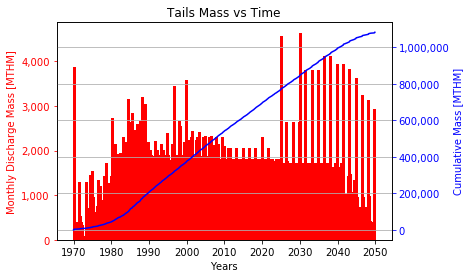
\includegraphics[width=\textwidth]{./images/eu_future/tails.png}
	\end{center}
	\caption{Timeseries of Tails Mass in the \gls{EU}.}
	\label{fig:eu_tail}
\end{minipage}
\hspace{.5cm}
\begin{minipage}[b]{.45\linewidth}
	\centering
	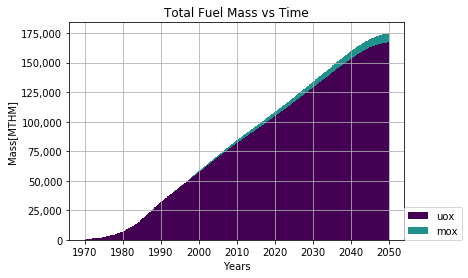
\includegraphics[width=\textwidth]{./images/eu_future/total_fuel.png}
	\caption{Timeseries of Total Fuel Usage in \gls{EU}.}
	\label{fig:eu_fuel}
\end{minipage}
\end{figure}
\end{frame}

\begin{frame}

\begin{figure}[htbp!]
	\begin{center}
			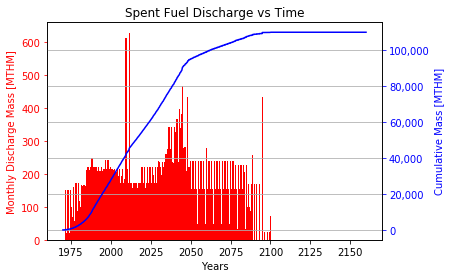
\includegraphics[scale=0.7]{./images/eu_future/snf_discharge.png}
	\end{center}
	\caption{Timeseries of Used Nuclear Fuel in \gls{EU}.}
	\label{fig:eu_snf}
\end{figure}

\end{frame}

\subsection{French Transition Scenario ~2160}

\begin{frame}
	\frametitle{SFR Deployment with Legacy UNF}
	\begin{itemize}
		\item Reprocessing UNF from all EU nations can start approx. 202 SFRs.
		\item Two generations of 66GWe SFRs = 220 SFRs
		\item Breeding Ratio of SFRs over one. ($\frac{23.95}{22.0} = 1.088$)
		\item Initial Pu loading of $4.9$ tons for ASTRID-type SFR \cite{varaine_pre-conceptual_2012}.
		\item $\frac{Pu \ from \ legacy \ \gls{UNF}}{4.9} \approx 202$
	\end{itemize}
\end{frame}

\begin{frame}
	\frametitle{Frech Transition Results}
	
\begin{table}[h]
	\centering
	\scalebox{0.86}{
		\begin{tabular}{ccc}
			\hline
			\textbf{Category} & \textbf{Unit} & \textbf{Value}  \\ \hline
			Total MOX used & MTHM & 63,820  \\ 
			Total \glspl{SFR} Deployed & & 220 \\ 
			Total Plutonium Reprocessed & MTHM & 15,230 \\ 
			Total \gls{ASTRID} fuel from UOX Waste & MTHM & 3,056  \\ 
			Total \gls{ASTRID} fuel from MOX Waste & MTHM  & 60,763 \\ 
			Total Tails used & MTHM & 49,779 \\ 
			Total legacy UNF reprocessed & MTHM & 56,584 \\ 
			Total Reprocessed Uranium Stockpile & MTHM & 184,789 \\ 
			Total Raffinate & MTHM & 35,834 \\ \hline
		\end{tabular}}
		\caption {\gls{SFR} Simulation Results}
		\label{tab:sfr_sim_result}
\end{table}

\end{frame}

\begin{frame}
	\frametitle{Material Flow in French Transition Scenario}
	
\begin{figure}[htbp!]
\begin{minipage}[b]{.45\linewidth}
	\begin{center}
		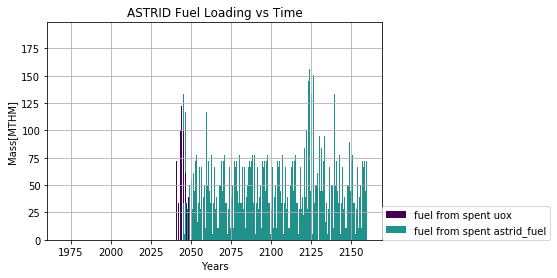
\includegraphics[width=\textwidth]{./images/french-transition/where_fuel.png}
	\end{center}
	\caption{Timeseries of fuel loaded into \glspl{SFR}, separated by origin}
	\label{fig:fuel}
\end{minipage}
\hspace{.5cm}
\begin{minipage}[b]{.45\linewidth}
	\centering
		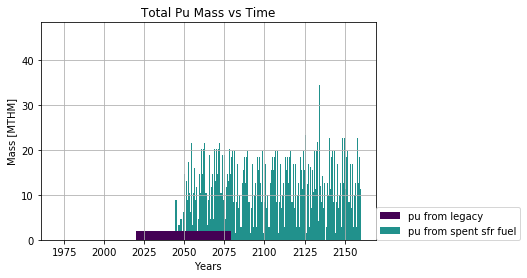
\includegraphics[width=\linewidth]{./images/french-transition/pu.png}
	\caption{Separated plutonium discharge from Reprocessing Plant}
	\label{fig:pu_no_cum}
\end{minipage}
\end{figure}

\end{frame}

\begin{frame}
	\frametitle{Material Flow in French Transition Scenario}
	
\begin{figure}[htbp!]
\begin{minipage}[b]{.45\linewidth}
	\begin{center}
		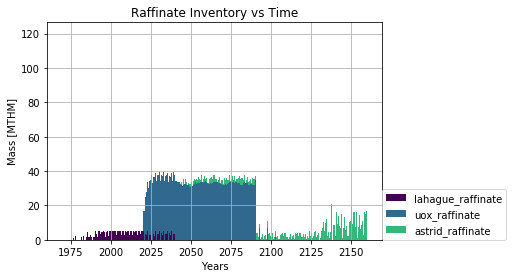
\includegraphics[width=\textwidth]{./images/french-transition/raffinate.png}
	\end{center}
	\caption{Timeseries of raffinate discharge from reprocessing plants}
	\label{fig:fuel}
\end{minipage}
\hspace{.5cm}
\begin{minipage}[b]{.45\linewidth}
	\centering
		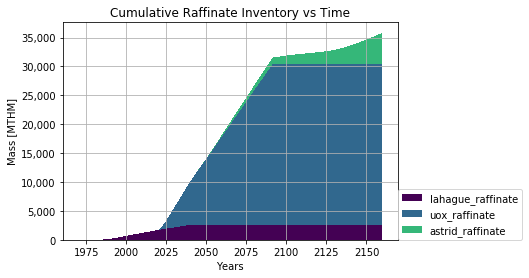
\includegraphics[width=\linewidth]{./images/french-transition/raffinate_cum.png}
	\caption{Cumulative raffinate inventory separated by origin}
	\label{fig:pu_no_cum}
\end{minipage}
\end{figure}

\end{frame}